\section{Cavern rock and EM debris}

\paragraph{Cavern rock (D7).} Muons running inside the rock near its surface ($1.6\times10^9$/spill; only
$\sim1.2\times10^5$ come back into the cavern) undergo DIS in concrete (\texttt{g4rock}: charged hadrons escape from
the top $\sim30$\,cm, $n$/$\gamma$ from $\sim1$\,m). \src{docs/full_sim_inventory.md, docs/STATUS.md (2026-11-08/09)}
\begin{itemize}
\item Muon rock: $4.6\times10^9$ per 15\,y with $\ge2$ good tracks, best-pair IP $\ge12.6$\,m $\Rightarrow$ 0 selected.
Neutrino rock: 12.4 interactions/spill, $3.2\times10^3$ per 15\,y with $\ge2$ good tracks, IP $\ge6.8$\,m $\Rightarrow$ 0.
\item Single tracks: the muon rock puts $1.84\times10^4$ good tracks per spill into SST1 (mostly hadrons and
electrons), comparable to the $\sim3\times10^4$ direct muons. In the combinatorial term: 0.023 per 15\,y after the veto.
\item \est{} The rock zero is 2.2\,M draws for $1.57\times10^{14}$ interactions per 15\,y: statistically only
$<1.6\times10^8$; it rests on geometry (a vertex must point back within 0.1\,m).
\end{itemize}

\paragraph{EM debris (B2, D12).} Electrons and photons from the shield end reaching the veto planes as accidental hits.
On the Nov-4 parents ($2\times10^5$ muons): $1.19\times10^9$ $e/\gamma$ per spill out of MS7; at the UBT
$5.2\times10^6$ $e$ + $2.5\times10^7$ $\gamma$ per spill. Effect on \texttt{D6\_straw\_mod}: combinatorial 0.014 $\to$
0.003 (more vetoes), signal loss $6.4\,\%\to7.5\,\%$. Behind 1\,m of iron 7.5--23\,\% of the muons carry an $e^\pm$
$>1$\,MeV (Fig.~\ref{fig:debris}); the field changes it by $\le5\,\%$. Open: debris in time with its muon, delta rays
in the planes, debris at the cavern-wall bounce points (D14). \src{docs/STATUS.md (31 Oct, 2026-11-10 night)}

\begin{figure}[h]
\centering
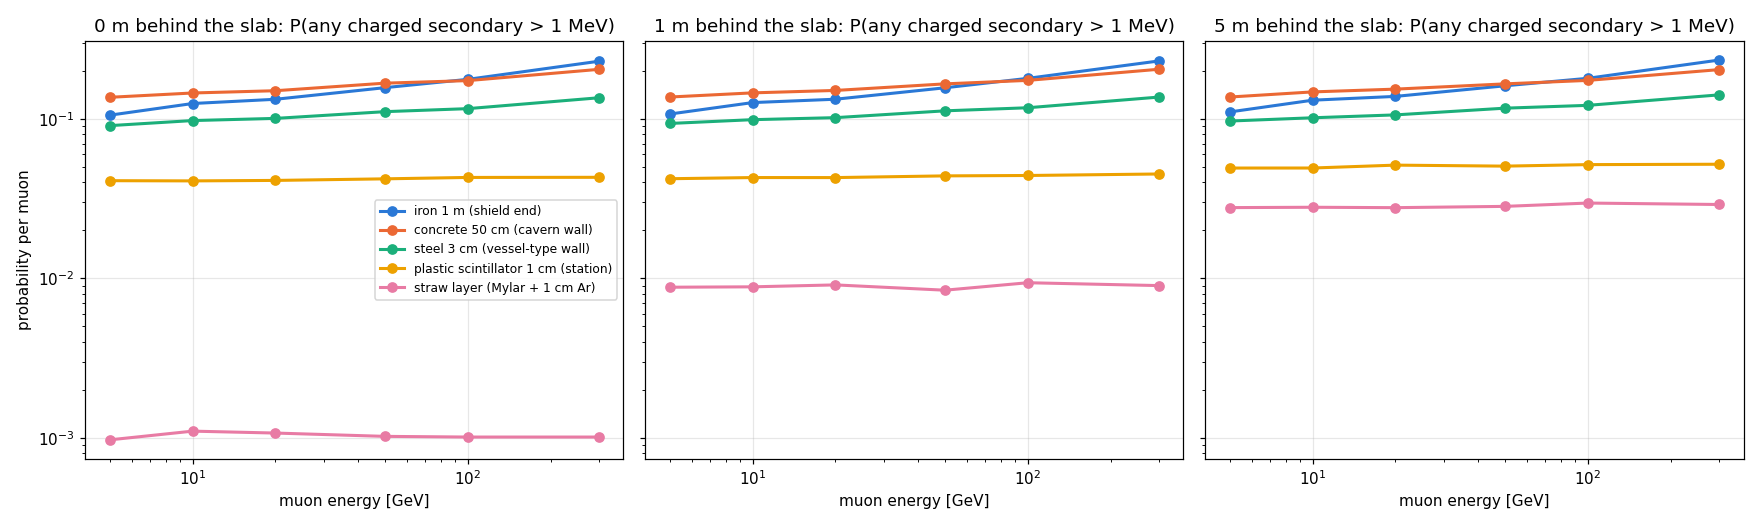
\includegraphics[width=\linewidth]{em_debris.png}
\caption{Probability of a charged secondary $>1$\,MeV behind an iron slab vs muon energy, at 0, 1 and 5\,m.
\src{lhcb_data .../results/em_debris/em_debris.png}}
\label{fig:debris}
\end{figure}
